\begin{enumerate}

\item A counter is constructed with three $D$ flip-flops. The input-output pairs are named $\brak{D_0, Q_0}$, $\brak{D_1, Q_1}$, and $\brak{D_2, Q_2}$, where the subscript $0$ denotes the least significant bit. The output sequence is desired to be the Gray-code sequence $000, 001, 011, 010, 110, 111, 101$, and $100$, repeating periodically. Note that the bits are listed in the $Q_2$  $Q_1$  $Q_0$ format. The combinational logic expression for $D_1$ is
\hfill(GATE-EE2021,37)

\begin{enumerate}
    \item $Q_2 Q_1 Q_0$
    \item $Q_2 Q_0 + Q_1 \Bar{Q_0}$
    \item $\Bar{Q_2} Q_0 + Q_1 \Bar{Q_0}$
    \item $Q_2 Q_1 + \Bar{Q_2} \Bar{Q_1}$
\end{enumerate}


\item The propagation delay of the exclusive- OR(XOR) gate in the circuit in the figure is $3$ ns. The propagation delay of all the flip-flops is assumed to be zero. The Clock(clk) frequency provided to the circuit is $500$ MHz.

	\begin{figure}[H]
    \centering
    \input{figs/figggss.tex}
    \caption{Propagation Delay}
	\label{fig:PropagationDelay}
\end{figure}
Starting from the initial value of the flip-flop outputs $Q2Q1Q0 =1 1 1$ with $D2=1$,the minimum number of triggering clock edges after which the flip-flop outputs $Q2Q1Q0$ becomes 1 0 0\emph (in integer) is \line(10,0){15}

\hfill(GATE-EC2021,46)


\item The maximum clock frequency in MHz of a 4-stage ripple counter, utilizing flip-flops, with each flip-flop having a propagation delay of 20 ns, is \rule{1cm}{0.10mm}. (round off to one decimal place)
\label{gate-ee-2022-29}
\hfill (GATE EE 2022)

\item The digital circuit shown \rule{1cm}{0.15mm}
\begin{center}
\begin{tikzpicture}
\ctikzset{                                   
logic ports=ieee,                   
logic ports/scale=0.5               
}                                    
\draw(-1.3,-0.56)node[nor port,anchor=out](x) {};  
%Drawing flip-flops
\draw (-1.3,-1.3) rectangle (0,0);
\draw(-1,-0.6) node{$D$};
\draw(-2,-1.1) node{$D_0$};
\draw(-0.2,-0.6) node{$Q$};
\draw(0.7,-1.3) rectangle (2,0);
\draw(1,-0.6) node{$D$};
\draw(1.8,-0.6) node{$Q$};
\draw(2.7,-1.3) rectangle (4,0);
\draw(3,-0.6) node{$D$};
\draw(3.8,-0.6) node{$Q$};
%connecting them
\draw(0,-0.6) -- (0.7,-0.6);
\draw(2,-0.6) -- (2.7,-0.6);
\draw(4,-0.6) -- (4.35,-0.6);
%drawing clk
\draw(-1.5,-2) node[above]{$CLK$} -- (3.35,-2);
%connecting clk 
\draw(-0.65,-2) -- (-0.65,-1.3);
\draw(1.35,-2) -- (1.35,-1.3);
\draw(3.35,-2) -- (3.35,-1.3);
\draw(3.35,-2) -- (4,-2);
%drawing clk edges
\draw(-0.5,-1.3) -- (-0.65,-1.1) -- (-0.8,-1.3);
\draw(1.2,-1.3) -- (1.35,-1.1) -- (1.5,-1.3);
\draw(3.2,-1.3) -- (3.35,-1.1) -- (3.5,-1.3);
%drawing Q2,Q1,Q0
%\draw(0.35,-0.6) --(0.35,0.2);
\draw(2.35,-0.6) --(2.35,0.3);
\draw(4.35,-0.6) --(4.35,0.9);
\draw(4.35,0.9) -- (-3,0.9);
\draw(2.35,0.3) -- (-2.5,0.3);
\draw(x.in 2) -|(-3,-0.7)to[short](-3,0.9);
\draw(x.in 1) -|(-2.5,-0.3)to[short](-2.5,0.3);
\draw(0.35,-0.3)node{$Q0$};
\draw(2.35,-0.35)node{$Q1$};
\draw(4.6,-0.35)node{$Q2$};
\end{tikzpicture}
\end{center}
\begin{enumerate}[label=(\Alph*)]
    \item is a divide-by-5 counter
    \item is a divide-by-7 counter
    \item is a divide-by-8 counter
    \item does not function as a counter due to disjoint cycles of states 
\end{enumerate}
\hfill{GATE IN 2022}
\item The propogation delay of the exclusive-OR(XOR) gate in the circuit in the figure is 3ns.The propogation delay of all the flip-flops is assumed to be zero.The clock(Clk) frequency provided to the circuit is 500MHz.
\label{prob:gate-ec-46.2021}
\hfill (GATE EC 2021)

\begin{tikzpicture}
\ctikzset{                                   
logic ports=ieee,                   
logic ports/scale=0.5               
}                                    
\draw(-1.3,-0.56)node[xor port,anchor=out](x) {};  
%Drawing flip-flops
\draw (-1.3,-1.3) rectangle (0,0);
\draw(-1,-0.6) node{$D2$};
\draw(0.7,-1.3) rectangle (2,0);
\draw(1,-0.6) node{$D1$};
\draw(2.7,-1.3) rectangle (4,0);
\draw(3,-0.6) node{$D0$};
%connecting them
\draw(0,-0.6) -- (0.7,-0.6);
\draw(2,-0.6) -- (2.7,-0.6);
\draw(4,-0.6) -- (4.35,-0.6);
%drawing clk
\draw(-1.5,-2) node[above]{$clk$} -- (3.35,-2);
%connecting clk 
\draw(-0.65,-2) -- (-0.65,-1.3);
\draw(1.35,-2) -- (1.35,-1.3);
\draw(3.35,-2) -- (3.35,-1.3);
%drawing clk edges
\draw(-0.5,-1.3) -- (-0.65,-1.1) -- (-0.8,-1.3);
\draw(1.2,-1.3) -- (1.35,-1.1) -- (1.5,-1.3);
\draw(3.2,-1.3) -- (3.35,-1.1) -- (3.5,-1.3);
%drawing Q2,Q1,Q0
\draw(0.35,-0.6) --(0.35,0.3);
\draw(2.35,-0.6) --(2.35,0.35);
\draw(4.35,-0.6) --(4.35,0.9);
\draw(4.35,0.9) -- (-3,0.9);
\draw(0.35,0.3) -- (-2.5,0.3);
\draw(x.in 2) -|(-3,-0.7)to[short](-3,0.9);
\draw(x.in 1) -|(-2.5,-0.3)to[short](-2.5,0.3);
\draw(0.35,0.5)node{$Q2$};
\draw(2.35,0.45)node{$Q1$};
\draw(4.35,1)node{$Q0$};
\end{tikzpicture}

Starting from the initial value of the flip-flop outputs $Q2Q1Q0 =111$ with $D2=1$,the minimum number of triggering clock edges after which the flip-flop outputs $Q2Q1Q0$ becomes 1 0 0\emph{(in integer)} is \line(1,0){12.5} 

\item  
\label{prob:gate IN 17}
For the $3$-bit binary counter shown in the figure, the output increments at every positive 
transition in the clock (CLK). Assume ideal diodes and the starting state of the counter as 
$000$. If output high is $1 V$ and output low is $0 V$, the current $I$(in mA) flowing through the 
$50 \Omega$ resistor during the $5$th clock cycle is (up to one decimal place)
\hfill(GATE IN 2018)
\begin{figure}[H]
\centering
\includegraphics[width=\columnwidth]{ide/7474/figs/pic.png}
\caption{circuit}
\label{fig:lcd}
\end{figure}
\item
\label{prob:gate CS 22}
Consider the sequential circuit shown in the figure, where both flip-flops used are positive
    edge-triggered D flip-flops.
\begin{figure}[H]
        \centering      
        \includegraphics[width=\columnwidth]{ide/7474/figs/wert.jpg}
        \caption{ckt}    
        \label{fig:wert}
    \end{figure}

    \item The number of states in the state transition diagram of this circuit that have a transition back to the same state on some value of ''in'' is \rule{30pt}{1pt}.
   \hfill(GATE IN 2018)
   \item The synchronous sequential circuit shown below works at a clock frequency of $1 GHz$. The throughput, in $Mbits/s$,and the latency, in $ns$, respectively, are 
\begin{figure}[H]
    \centering
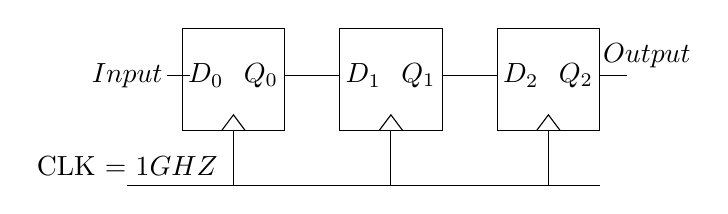
\begin{tikzpicture}
\ctikzset{                                  
    logic ports=ieee,                   
    logic ports/scale=0.5               
}                                    

% Drawing flip-flops
\draw (-1.3,-1.3) rectangle (0,0);
\draw(-1,-0.6) node{$D_0$};
\draw(-0.3,-0.6) node{$Q_0$};
\draw(0.7,-1.3) rectangle (2,0);
\draw(1,-0.6) node{$D_1$};
\draw(1.7,-0.6) node{$Q_1$};
\draw(2.7,-1.3) rectangle (4,0);
\draw(3,-0.6) node{$D_2$};
\draw(3.7,-0.6) node{$Q_2$};

% Connecting them
\draw(0,-0.6) -- (0.7,-0.6);
\draw(2,-0.6) -- (2.7,-0.6);
\draw(4,-0.6) -- (4.35,-0.6);
\draw(-1.2,-0.6) -- (-1.5,-0.6);

% Drawing clk
\draw(-2,-2) node[above]{CLK = $1GHZ$ } -- (3.35,-2);

% Connecting clk
\draw(-0.65,-2) -- (-0.65,-1.3);
\draw(1.35,-2) -- (1.35,-1.3);
\draw(3.35,-2) -- (3.35,-1.3);
\draw(3.35,-2) -- (4,-2);

% Drawing clk edges
\draw(-0.5,-1.3) -- (-0.65,-1.1) -- (-0.8,-1.3);
\draw(1.2,-1.3) -- (1.35,-1.1) -- (1.5,-1.3);
\draw(3.2,-1.3) -- (3.35,-1.1) -- (3.5,-1.3);

% Drawing Q2, Q1, Q0
\draw(0.35,-0.3)node{};
\draw(2.35,-0.35)node{};
\draw(4.6,-0.35)node{$ Output $};
\draw(-2,-0.6)node{$ Input $};
\end{tikzpicture}
\label{prob:gate EC 2023}
\end{figure}

    \begin{enumerate}
        \item $1000, 3$
         \item $333.33, 1$
          \item $2000, 3$
           \item $333.33 , 3$
    \end{enumerate}
\hfill(GATE EC 2023)
\label{prob:GATE EC 2023}
\item In a given sequential circuit, initial states are $Q1 = 1$ and $Q2 = 0$. For a clock frequency of $1 MHz$, the frequency of signal $Q2$ in kHz, is(rounded off to the nearest integer)
    
\begin{figure}[H]
    \centering
\begin{tikzpicture}              

%Drawing flip-flops
\draw (1.6,1.9) node {D Flip Flop};
\draw (0,0)--(3,0)--(3,4)--(0,4)--(0,0);
\draw(0.5,3.5) node{$D_1$};
\draw(2.5,3.5) node{$Q_1$};
\draw(2.5,0.5) node{$\bar{Q_1}$};
\draw(3.1,0.5) node{$\circ$};

\draw (8.6,1.9) node {D Flip Flop};
\draw(7,0)--(7,4)--(10,4)--(10,0)--(7,0);
\draw(7.5,3.5) node{$D_2$};
\draw(9.5,3.5) node{$Q_2$};
\draw(9.5,0.5) node{$\bar{Q_2}$};
\draw(10.1,0.5) node{$\circ$};

%connecting them
\draw(3.2,0.5)--(4.0,0.5);
\draw(10.2,0.5)--(10.9,0.5);
\draw(7.0,3.5)--(6.0,3.5);
\draw(4.0,0.5) -- (6.0,3.5);
\draw(10.0,3.5) -- (10.9,3.5);
\draw(4.0,3.5) --(3.0,3.5);

\draw(-1.1,-1.2)-- (8.5,-1.2);

%drawing clk
\draw (-1.0,-1.7)node{CLK =1Mhz};


%connecting clk 
\draw(1.5,-1.2) -- (1.5,0.0);
\draw(8.5,-1.2) -- (8.5,0.0);

%drawing clk edges
\draw(1.1,0.0) -- (1.48,0.4) -- (1.9,0.0);
\draw(8.1,0.0) -- (8.48,0.4) -- (8.9,0.0);

% Drawing Q2, D1,
\draw(10.9,3.5)--(10.9,5.4);
\draw(10.9,5.4)--(-1.0,5.4);
\draw(-1.0,5.4)--(-1.0,3.5);
\draw(0,3.5)--(-1.0,3.5);
\end{tikzpicture}
\end{figure}
\hfill(GATE EC 2023)

\item Neglecting the delays due to the logic gates in the circuit shown in figure, the 
decimal equivalent of the binary sequence $[ABCD]$ of initial logic states, which will not change with clock, is $\underline{\hspace{2cm}}$.\\

\hfill{(EE GATE 2023)}\\

\begin{figure}[H]
 \centering
\includegraphics[width=\columnwidth]{ide/7474/figs/Gate_question.png}
\caption{Neglecting the delays}
\label{fig:Gate_question.png}
\end{figure}

\item 
Consider a sequential digital circuit consisting of T flip-flops and D flip-flops as shown in the figure. CLKIN is is the clock input to the circuit. At the beginning,Q1,Q2 and Q3 have values 0,1 and 1, respectively.
\hfill(GATE CS2023,43)

\begin{figure}[H]
\centering
\input{ide/7474/figs/fig.tex}
\caption{Flip-Flop}
\label{fig:Flip-Flop}
\end{figure}
Which of the given values of \((Q_1, Q_2, Q_3)\) can NEVER be obtained with this digital circuit?
\begin{enumerate}
    
    \item ${(0,0,1)}$
    \item ${(1,0,0)}$
    \item ${(1,0,1)}$
    \item ${(1,1,1)}$
\end{enumerate}
\item In the circuit shift, the initial binary content of the shift register A $1101$ and that of shift register B is $1010$ The shift registers are positive edge triggered, and the gates have no delay.
when the shift control is high,what will be the binary content of the shift registers $A$ and $B$ after clock pulses?

\hfill{(GATE IN 2023)}

\begin{figure}[H]
\centering
\includegraphics[width=\columnwidth]{ide/7474/figs/Gate.png}
\caption{circuit Digram}
\label{fig:cricuit Digram}
\end{figure}

\begin{enumerate}
\item $A= 1101,B=1101$
\item $A=1110 ,B=1001$
\item $A=0101 ,B=1101$
\item $A=1010 ,B=1111$
\end {enumerate}
\item For the circuit shown, the clock frequency is $f_0$ and the duty cycle is $25\%$. For the signal at the Q output of the Flip-Flop,\underline{\hspace{20pt}}.\hfill(GATE EC 2022)
		\begin{figure}[h]
			\centering
			\includegraphics[width=\columnwidth]{ide/7474/figs/gate_image_new.jpg}
			\caption{Circuit}
			\label{fig:new_gate}
		\end{figure}
			\begin{enumerate}
			\item frequency is $\frac{{f_0}}{4}$ and duty cycle is $50\%$
			\item frequency is $\frac{{f_0}}{4}$ and duty cycle is $25\%$
			\item frequency is $\frac{{f_0}}{2}$ and duty cycle is $50\%$
			\item frequency is ${f_0}$ and duty cycle is $25\%$
		\end{enumerate}
\item In the circuit shown, the initial binary content of shift register A is 1101 and that of shift register B is 1010.The shift registers are positive edge triggered, and the gates have no delay.

When the shift control is high,what will be the binary content of the shift registers A and B after four clock pulses?
\hfill{(Gate IN 2023)}

		\begin{figure}[H]
			\includegraphics[width=\columnwidth]{figs/shift.jpeg}
			\caption{Shift register}
			\label{figs:fig1}
		\end{figure}
\begin{enumerate}
  \item A=1101,B=1101
  \item A=1110,B=1001
  \item A=0101,B=1101
  \item A=1010,B=1111
\end{enumerate}
\item The digital circuit shown in \figref{fig:GATEIN202236.png}
\begin{figure}[H]
  \centering
  \includegraphics[width=\columnwidth]{ide/7474/figs/GATEIN202236.png}
  \caption{}
  \label{fig:GATEIN202236.png}
\end{figure}
 \begin{enumerate}
 \item is a divide-by-$5$ counter
 \item is a divide-by-$7$ counter
 \item is a divide-by-$8$ counter
 \item does not function as a counter due to disjoint cycles of states 
\end{enumerate}
\hfill(GATE-IN-2022)

 \item Given below is the diagram of a synchronous sequential circuit with one $J-K$ flip-flop and one $T$ flip-flop with their outputs denoted as $A$ and $B$ respectively, with $J_{A}=\brak{A^{\prime}+B^{\prime}}$, $K_{A}=(A+B)$ and $T_{B}=A$.Starting from the initial state $\brak{AB=00}$, the sequence of states $\brak{AB}$ visited by the circuit is
\hfill(GATE-IN2021)
	      \begin{figure}[H]
		      \centering
		      \input{figs/jkff.tex}
		      \caption{synchronous}
		      \label{}
	      \end{figure}
		  \begin{enumerate}
          \item $00 \rightarrow 01 \rightarrow 10 \rightarrow 11 \rightarrow 00 
          \dots $
          \item $00 \rightarrow 10 \rightarrow 01 \rightarrow 11 \rightarrow 00 
          \dots $
          \item $00 \rightarrow 10 \rightarrow 11 \rightarrow 01 \rightarrow 00 \dots $
          \item $00 \rightarrow 01 \rightarrow 11 \rightarrow 00 \dots $
      \end{enumerate}
  \item Consider the $D$-Latch shown in the figure, which is transparent when its clock input $CK$ is high and has zero propagation delay. In the figure, the clock signal $CLK1$ has $50\%$ duty cycle and $CLK2$ is a one fifth period delayed version of $CLK1$. The duty cycle at the output of the latch in percentage is.
  \hfill(GATE-EC2017)
	      \begin{figure}[h!]
		      \begin{center}
			      \input{ide/7474/figs/fig22245.tex}
			      \caption{}
		      \end{center}
	      \end{figure}
\item A $4$-bit shift register circuit configured for right-shift operation, i.e.\\ $D_{in} \rightarrow A, A \rightarrow B, B \rightarrow C, C \rightarrow D$, is shown. If the present state of the shift register is $ABCD = 1101$, the number of clock cycles required to reach the state $ABCD = 1111$ is

\hfill (GATE-EC 2017)
\begin{figure}[H]
    \centering
	\input{ide/7474/figs/fig22246.tex}
 	\caption{}
\end{figure}

\item In the circuit shown, the clock frequency, i.e., the frequency of the clk signal, is 12 KHz. The frequency of the signal at $\mathbf{Q2}$ is $\underline{\hspace{18pt}}$ KHz.
		\hfill(GATE-EC2019,25)
%%\end{enumerate}
		\begin{figure}[H]
			\input{ide/7474/figs/fig1.tex}
			\caption{Circuit Daigram}
		\end{figure}

 \item The circuit shown in the figure below uses ideal positive edge-triggered synchronous $J-K$ flip flops with outputs $X$ and $Y$. If the initial state of the output is $X=0$ and $Y=0$ just before the arrival of the first clock pulse, the state of the output just before the arrival of the second clock pulse is
              \hfill(GATE-IN2019,12)
\begin{figure}[H]
    \centering
    \input{ide/7474/figs/fig7.tex}
   

\end{figure}
\begin{enumerate}
    \item $X=0$, $Y=0$
    \item $X=0$, $Y=1$
    \item $X=1$, $Y=0$
    \item$X=1$, $Y=1$
\end{enumerate}

\item Consider a $4$-bit counter constructed out of four flip-flops.It is formed by connecting the J and K inputs to logic high and feeding the Q output to the clock input of the following flip-flop (see the figure).The input signal to the counter is a series of square pulses and the change of state is triggered by the falling edge.At time t=t0 the outputs are in logic low state (Q0 = Q1 = Q2 = Q3 = 0).Then at t=t1,the logic state of the outputs is 
		               \hfill(GATE-PH2020,30)
\begin{figure}[H]
    \centering
\input{ide/7474/figs/fig10.tex}
    \caption{Ripple Counter}
   
    \end{figure}
\begin{enumerate}
\item  Q0 = 1, Q1 = 0, Q2 = 0 and Q3 = 0 
\item  Q0 = 0, Q1 = 0, Q2 = 0 and Q3 = 1
\item  Q0 = 1, Q1 = 0, Q2 = 1 and Q3 = 0
\item  Q0 = 0, Q1 = 1, Q2 = 1 and Q3 = 1
\end{enumerate}




\item Two T-flip flops are interconnected as shown in the figure. The present state of the flip flops are: A = 1, B = 1. The input x is given as $1, 0, 1$ in the next three clock cycles. The decimal equivalent of $\brak{ABy}_{2}$ with A being the MSB and y being the LSB, after the $3_{rd}$ clock cycle is $\underline{\hspace{2cm}}$.
\hfill{\brak{GATE \enspace IN2020-40}}
\begin{figure}[H]
\input{ide/7474/figs/fig15.tex}
\caption{Circuit Diagram}

\end{figure}

\item For the components in the sequential circuit shown below, $t_{\text{pd}}$ is the propagation delay, $t_{\text{setup}}$ is the setup time, and $t_{\text{hold}}$ is the hold time. The maximum clock frequency (rounded off to the nearest integer) at which the given circuit can operate reliably is \underline{\hspace{1cm}}MHZ.
\hfill{\brak{GATE \enspace EC2020-50}}

\begin{figure}[H]
\input{ide/7474/figs/fig16.tex}
\caption{Circuit Diagram}

\end{figure}

\item A 2-bit synchronous counter using two J-K flip flops is shown. The expression for the inputs to the J-K flip flops are also shown in the figure. The output sequence of the counter starting from $Q_{1}Q_{2} = 00$ is
\hfill{GATE-IN2018,44}
\begin{figure}[!ht]
\centering
\input{ide/7474/figs/gate_in_2018_44.tex}
\label{fig:gate_in_2018_44}
\end{figure}
\begin{enumerate}[label=\Alph*.]
\item $00 \rightarrow 11 \rightarrow 10 \rightarrow 01 \rightarrow 00 \hdots $
\item $00 \rightarrow 01 \rightarrow 10 \rightarrow 11 \rightarrow 00 \hdots $
\item $00 \rightarrow 01 \rightarrow 11 \rightarrow 10 \rightarrow 00 \hdots $
\item $00 \rightarrow 10 \rightarrow 11 \rightarrow 01 \rightarrow 00 \hdots $
\end{enumerate}

 \item Which of the following statements is true about digital circuits shown in the figure 
 \hfill{(Gate EE-2018,36)}

\begin{circuitikz}


\draw (0,0)node[left]{$f_{in}$} to[short,*-] (8,0);
\draw (0.5,0) to (0.5,1);
\draw (0.5,1) to (1,1);
\draw (1,0.65) to (1,3);
\draw (1,3) to (3,3);
\draw (3,3) to (3,0.65);
\draw (3,0.65) to (1,0.65);
\draw (1,2.65) node[right]{D}to (0.5,2.65);
\draw (0.5,2.65) to (0.5, 5);
\draw (0.5,5) to (4,5);
\draw (3,2.65) node[left]{Q}to (5,2.625) node[right]{D};
\draw (5,0.65) to (5,3);
\draw (5,3) to (7,3);
\draw (7,3) to(7,0.65);
\draw (5,0.65) to (7,0.65);
\draw (4,0) to (4,1);
\draw (4,1) to (5,1);
\draw (7,2.65) node[left]{Q} to (9,2.65) node[right]{D};
\draw (9,0.65) to (9,3);
\draw (9,3) to (11,3);
\draw (11,3) to (11,0.65);
\draw (11,0.65) to (9,0.65);
\draw (8,0) to (8,1);
\draw (8,1) to (9,1);
\draw (11,2.65) node [left]{Q} to [short,-*](12,2.65) node[right]{$f_{out}$};
\draw (8,2.65) to (8,4.5);
\draw (8,4.5) to (6.25,4.5);
\draw (11.5,2.65) to (11.5,5.5);
\draw (11.5,5.5) to (6.25,5.5);
\draw (1,1.25) to (1.25,1);
\draw (1.25,1) node[right]{C} to (1,0.75);
\draw (5,1.25) to (5.25,1);
\draw (5.25,1) node[right]{C} to (5,0.75);
\draw (9,1.25) to (9.25,1);
\draw (9.25,1) node[right]{C} to (9,0.75);
% nand
\draw (4,5) node[rotate=180,nand port,scale=1.77](nand){};
\end{circuitikz}

					 
\begin{enumerate}
\item [(A)]It can be used  for dividing the input frequency by $3$ .
\item [(B)] It can be used  for dividing the input frequency by $5$ .
\item [(C)] It can be used  for dividing the input frequency by $7$ .
\item [(D)] It cannot be reliably used as frequency divider due to 
 disjoint internal cycles .
 \end{enumerate}



 \item In the circuit shown below, a positive edge-triggered $D$ Flip-Flop is used for sampling input data $D_{in}$ using clock $CK$. The $XOR$ gate outputs $3.3$ volts for logic HIGH and $0$ volts for logic LOW levels. The data bit and clock periods are equal and the value of $\triangle T/ T_{CK} = 0.15 .$, where the parameters $\triangle T$ and $T_{CK}$ are shown in the figure. Assume that the Flip-Flop and the $XOR$ gate are ideal.
\hfill (GATE-EC 2018,46)
\begin{figure}[H]
			\input{ide/7474/figs/ckt.tex}
			\caption{Circuit Daigram}
\end{figure}
 If the probability of input data bit ($D_{in}$) transition in each clock period is $0.3$, the average
    value (in volts, accurate to two decimal places) of the voltage at node $X$, is $..........$.
    
 \item Assume that all the digital gates in the circuit shown in the figure are ideal,the resistor $R$=$10k\Omega $ and the supply voltages is $5V$.The $D$ flip-flops $D_1,D_2,D_3,D_4$ and $D_5$ are intialized with logic values $0,1,0,1,$ and $0,$ respectively.The clock has a $30\%$ duty cycle.
 
    \begin{circuitikz}[scale=0.8]

      \tikzset{flipflop AB/.style={flipflop,
    flipflop def={t1=D,t6=Q,td={\texttt{CLK}}},
 }}
     \draw(0,0) node[flipflop AB](D1){D1} ;
     \draw(3,0) node[flipflop AB](D2){D2};
     \draw(6,0) node[flipflop AB](D3){D3};
     \draw(9,0) node[flipflop AB](D4){D4};
     \draw(12,0) node[flipflop AB](D5){D5};
     \draw (D1.pin 6) --  (D2.pin 1);
     \draw (D2.pin 6) --  (D3.pin 1);
     \draw (D3.pin 6) --  (D4.pin 1);
     \draw (D4.pin 6) --  (D5.pin 1);
     \draw (15.2,5) node[or port] (or) {};
     \draw (or.in 1) node[left]{};
     \draw (or.in 2) node[left]{};
     \draw (or.out) node[right]{};
     \draw (D5.pin 6) -- (or.in 2);
     \draw (-3,1.05) -- (D1.pin 1);
     \draw (-3,1.05) -- (-3,-3);
     \draw (-3,-3) --   (13.45,-3);
     \draw (13.4,-3) -- (D5.pin 6);
     \draw (7.3,5.3) -- (or.in 1);
     \draw (7.3,1.05) -- (7.3,5.25);
     \draw (0,-2) -- (0,-1.5);
     \draw (0,-2) -- (3,-2);
     \draw (3,-2) -- (6,-2);
     \draw (6,-2) -- (9,-2);
     \draw (9,-2) -- (12,-2);
     \draw (15.4,5) to[R, l=$10\, \text{k}\Omega$] (15.4,0);
     \draw (15.38,0) node[ground]{};
     \draw (-1,-2) node[left](q){$Clock$};
     \draw (q) -- (0,-2);
\end{circuitikz}

The average power dissipated $\brak {in mW}$  in the resistor R is 
\hfill{(GATE EC 2016)}
 












\end{enumerate}
\item Consider the following  $\#$, with the following:\\
$x\#0=x$, $x\#1 = \overline{x}$, $x\#x = 0$ and $x\#\overline{x}=1$. Then $x\#y$ is equivalent to\\
\hfill 
\\
\begin{minipage}{0.99\textwidth}
    \textbf{(A)} $x\overline{y} + \overline{x}y$
\end{minipage}
\hfill
\\
\begin{minipage}{0.99\textwidth}
    \textbf{(B)} $x\overline{y} + \overline{x}\overline{y}$
\end{minipage}
\hfill
\\
\begin{minipage}{0.99\textwidth}
    \textbf{(C)} $\overline{x}y + xy$
\end{minipage}
\hfill
\\
\begin{minipage}{0.99\textwidth}
    \textbf{(D)} $x{y} + \overline{x}\overline{y}$
\end{minipage}
\\

 

\end{enumerate}
